\chapter{Experiment}
\label{ch:experiment}

\section{Data Collection}
To evaluate proposed method. We use two group of stocks:
\begin{enumerate}
	\item Group 1: NASDAQ, S\&P500, DJI, DAX.
	
	\item Group 2: Exxon Mobil, Chervon.
\end{enumerate}

In each group, group members are highly correlated with each other (see \autoref{fig:nas_base} for group 1, \autoref{fig:exx_base} for group 2).

\bigskip

We collect the daily quote data of those stocks from Yahoo Finance \cite{yf}.

\bigskip

\autoref{tab:raw-data} shows an example for data download from Yahoo.

\begin{table}[H]
	\caption{NASDAQ data download from Yahoo Finance.}
	\begin{tabular}{|c|c|c|c|c|c|}
		\hline
		\textbf{Date} & \textbf{Open} & \textbf{High} & \textbf{Low} & \textbf{Close} & \textbf{Volume} \\
		\hline
		1971-02-05    & 100.0000      & 100.0000      & 100.0000     & 100.0000       & 0               \\
		\hline
		1971-02-08    & 100.8399      & 100.8399      & 100.8399     & 100.8399       & 0               \\
		\hline
		1971-02-09    & 100.7600      & 100.7600      & 100.7600     & 100.7600       & 0               \\
		\hline
		1971-02-10    & 100.6900      & 100.6900      & 100.6900     & 100.6900       & 0               \\
		\hline
		1971-02-11    & 101.4499      & 101.4499      & 101.4499     & 101.4499       & 0               \\
		\hline
		...           & ...           & ...           & ...          & ...            & ...             \\
		\hline
		2024-05-01    & 15646.0898    & 15926.2197    & 15557.6396   & 15605.4804     & 5277790000      \\
		\hline
		2024-05-02    & 15758.1103    & 15862.7900    & 15604.7304   & 15840.9599     & 4901610000      \\
		\hline
		2024-05-03    & 16147.4804    & 16204.7099    & 16068.3398   & 16156.3300     & 4887310000      \\
		\hline
		2024-05-06    & 16208.5400    & 16350.0800    & 16197.8603   & 16349.2500     & 4460130000      \\
		\hline
		2024-05-07    & 16208.5000    & 16396.4589    & 16326.2109   & 16373.5625     & 2693650000      \\
		\hline
	\end{tabular}
	\label{tab:raw-data}
\end{table}

Date: The specific day when the trading occurred.

Open: The price of the stock index at the beginning of the trading day (USD).

High: The highest price reached by the stock index during the trading day (USD).

Low: The lowest price reached by the stock index during the trading day (USD).

Close: The price of the stock index at the end of the trading day (USD).

Volume: The total number of shares traded during the day (share).

\section{Data Pre-processing}
First, we fill forward all missing dates in the range from starting date to current
date. To smooth out the ups and downs in stock prices, we start by averaging the
values over a \textbf{14-day} period (see \autoref{tab:mva-data}). Then, we
calculate the percentage change for the next day (see \autoref{tab:pct-data}). When
building our model, we make sure to scale these percentage changes so they fall
between 0 and 1, using a standard min-max scaling method we get the result is \autoref{tab:nor-data}
for NASDAQ and \autoref{tab:nor2-data} for S\&P500.

\begin{equation}
	x_{\text{standarlized }}=\frac{x-\min (x)}{\max (x)-\min (x)}\label{normalized}
\end{equation}

Finally, we push all the processed data (\autoref{tab:nor-data} and
\autoref{tab:nor2-data}) to the Geometry Mean Not NaN block (\autoref{fig:gmnn}),
which will be the final input to feed for the model (see \autoref{tab:final-data}).

\begin{table}[H]
	\centering
	\caption{NASDAQ data after filling missing dates and applying Moving Average.}
	\begin{tabular}{|c|c|c|c|c|c|}
		\hline
		\textbf{Date} & \textbf{Open} & \textbf{High} & \textbf{Low} & \textbf{Close} & \textbf{Volume} \\
		\hline
		1971-02-18    & 101.3850      & 101.3850      & 101.3850     & 101.3850       & 6.2860e+7       \\
		\hline
		1971-02-19    & 101.4350      & 101.4350      & 101.4350     & 101.4350       & 6.2860e+7       \\
		\hline
		1971-02-20    & 101.3521      & 101.3521      & 101.3521     & 101.3521       & 6.2860e+7       \\
		\hline
		1971-02-21    & 101.2692      & 101.2692      & 101.2692     & 101.2692       & 6.2860e+7       \\
		\hline
		1971-02-22    & 101.1864      & 101.1864      & 101.1864     & 101.1864       & 6.2860e+7       \\
		\hline
		...           & ...           & ...           & ...          & ...            & ...             \\
		\hline
		2024-05-03    & 15729.2649    & 15846.3864    & 15614.3349   & 15750.9149     & 4.870674e+9     \\
		\hline
		2024-05-04    & 15787.2942    & 15904.3207    & 15680.9206   & 15815.0535     & 4.859489e+9     \\
		\hline
		2024-05-05    & 15845.3235    & 15962.2550    & 15747.5064   & 15879.1921     & 4.848303e+9     \\
		\hline
		2024-05-06    & 15903.3528    & 16020.1893    & 15814.0921   & 15943.3307     & 4.837117e+9     \\
		\hline
		2024-05-07    & 15952.1349    & 16067.8352    & 15870.7528   & 15988.7533     & 4.815941e+9     \\
		\hline
	\end{tabular}
	\label{tab:mva-data}
\end{table}

\begin{table}[H]
	\centering
	\caption{NASDAQ data after computing percentage change.}
	\begin{tabular}{|c|c|c|c|c|c|}
		\hline
		\textbf{Date} & \textbf{Open} & \textbf{High} & \textbf{Low} & \textbf{Close} & \textbf{Volume} \\
		\hline
		1971-02-19    & 0.000493      & 0.000493      & 0.000493     & 0.000493       & 0               \\
		\hline
		1971-02-20    & -0.000817     & -0.000817     & -0.000817    & -0.000817      & 0               \\
		\hline
		1971-02-21    & -0.000818     & -0.000818     & -0.000818    & -0.000818      & 0               \\
		\hline
		1971-02-22    & -0.000818     & -0.000818     & -0.000818    & -0.000818      & 0               \\
		\hline
		1971-02-23    & -0.000734     & -0.000734     & -0.000734    & -0.000734      & 0               \\
		\hline
		...           & ...           & ...           & ...          & ...            & ...             \\
		\hline
		2024-05-03    & 0.002734      & 0.002839      & 0.003883     & 0.003981       & -0.006248       \\
		\hline
		2024-05-04    & 0.003689      & 0.003656      & 0.004264     & 0.004072       & -0.002297       \\
		\hline
		2024-05-05    & 0.003676      & 0.003643      & 0.004246     & 0.004056       & -0.002302       \\
		\hline
		2024-05-06    & 0.003662      & 0.003629      & 0.004228     & 0.004039       & -0.002307       \\
		\hline
		2024-05-07    & 0.003067      & 0.002974      & 0.003583     & 0.002849       & -0.004378       \\
		\hline
	\end{tabular}
	\label{tab:pct-data}
\end{table}

\begin{table}[H]
	\centering
	\caption{NASDAQ data after normalizing.}
	\begin{tabular}{|c|c|c|c|c|c|}
		\hline
		\textbf{Date} & \textbf{Open} & \textbf{High} & \textbf{Low} & \textbf{Close} & \textbf{Volume} \\
		\hline
		1971-02-19    & 0.635564      & 0.635564      & 0.635564     & 0.635564       & 0.481983        \\
		\hline
		1971-02-20    & 0.606946      & 0.606946      & 0.606946     & 0.606946       & 0.481983        \\
		\hline
		1971-02-21    & 0.606932      & 0.606932      & 0.606932     & 0.606932       & 0.481983        \\
		\hline
		1971-02-22    & 0.606917      & 0.606917      & 0.606917     & 0.606917       & 0.481983        \\
		\hline
		1971-02-23    & 0.608753      & 0.608753      & 0.608753     & 0.608753       & 0.481983        \\
		\hline
		...           & ...           & ...           & ...          & ...            & ...             \\
		\hline
		2024-05-03    & 0.684514      & 0.686807      & 0.709619     & 0.711752       & 0.449510        \\
		\hline
		2024-05-04    & 0.705385      & 0.704658      & 0.717949     & 0.713747       & 0.470046        \\
		\hline
		2024-05-05    & 0.705089      & 0.704367      & 0.717554     & 0.713387       & 0.470019        \\
		\hline
		2024-05-06    & 0.704795      & 0.704079      & 0.717161     & 0.713029       & 0.469991        \\
		\hline
		2024-05-07    & 0.691800      & 0.689762      & 0.703062     & 0.687029       & 0.459228        \\
		\hline
	\end{tabular}
	\label{tab:nor-data}
\end{table}

\begin{table}[H]
	\centering
	\caption{S\&P500 data after normalizing.}
	\begin{tabular}{|c|c|c|c|c|c|}
		\hline
		\textbf{Date} & \textbf{Open} & \textbf{High} & \textbf{Low} & \textbf{Close} & \textbf{Volume} \\
		\hline
		1928-01-13    & 0.521913      & 0.521913      & 0.521913     & 0.521913       & 0.458965        \\
		\hline
		1928-01-14    & 0.490008      & 0.490008      & 0.490008     & 0.490008       & 0.458965        \\
		\hline
		1928-01-15    & 0.489934      & 0.489934      & 0.489934     & 0.489934       & 0.458965        \\
		\hline
		1928-01-16    & 0.489860      & 0.489860      & 0.489860     & 0.489860       & 0.458965        \\
		\hline
		1928-01-17    & 0.490609      & 0.490609      & 0.490609     & 0.490609       & 0.458965        \\
		\hline
		...           & ...           & ...           & ...          & ...            & ...             \\
		\hline
		2024-05-03    & 0.561882      & 0.562470      & 0.570750     & 0.574165       & 0.460139        \\
		\hline
		2024-05-04    & 0.572563      & 0.568649      & 0.577909     & 0.576782       & 0.455490        \\
		\hline
		2024-05-05    & 0.572467      & 0.568569      & 0.577788     & 0.576667       & 0.455481        \\
		\hline
		2024-05-06    & 0.572371      & 0.568490      & 0.577668     & 0.576552       & 0.455472        \\
		\hline
		2024-05-07    & 0.573196      & 0.563337      & 0.571300     & 0.561493       & 0.421249        \\
		\hline
	\end{tabular}
	\label{tab:nor2-data}
\end{table}

\begin{table}[H]
	\centering
	\caption{Combine NASDAQ and S\&P500 using GMNN block.}
	\begin{tabular}{|c|c|c|c|c|c|}
		\hline
		\textbf{Date} & \textbf{Open} & \textbf{High} & \textbf{Low} & \textbf{Close} & \textbf{Volume} \\
		\hline
		1928-01-13    & 0.521913      & 0.521913      & 0.521913     & 0.521913       & 0.458965        \\
		\hline
		1928-01-14    & 0.490008      & 0.490008      & 0.490008     & 0.490008       & 0.458965        \\
		\hline
		1928-01-15    & 0.489934      & 0.489934      & 0.489934     & 0.489934       & 0.458965        \\
		\hline
		1928-01-16    & 0.489860      & 0.489860      & 0.489860     & 0.489860       & 0.458965        \\
		\hline
		1928-01-17    & 0.490609      & 0.490609      & 0.490609     & 0.490609       & 0.458965        \\
		\hline
		...           & ...           & ...           & ...          & ...            & ...             \\
		\hline
		2024-05-03    & 0.620174      & 0.621537      & 0.636408     & 0.639268       & 0.454793        \\
		\hline
		2024-05-04    & 0.635514      & 0.633011      & 0.644135     & 0.641621       & 0.462711        \\
		\hline
		2024-05-05    & 0.635327      & 0.632836      & 0.643890     & 0.641394       & 0.462693        \\
		\hline
		2024-05-06    & 0.635141      & 0.632662      & 0.643647     & 0.641169       & 0.462675        \\
		\hline
		2024-05-07    & 0.629712      & 0.623353      & 0.633766     & 0.621098       & 0.439829        \\
		\hline
	\end{tabular}
	\label{tab:final-data}
\end{table}

We use the technique moving average that used sequence previous days movements to
predict the next day change, which is our target. This approach takes into account
the short-term trends in stock prices and uses time series indicators as features
to classify the trend.

\begin{figure}[H]
	\centering
	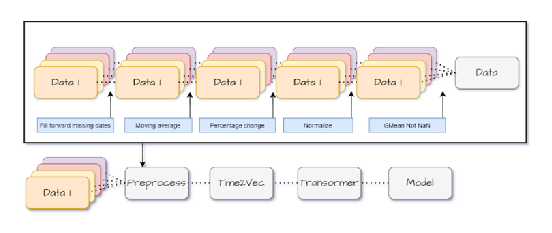
\includegraphics[width=1\linewidth]{images/pipeline.eps}
	\caption{Pre-processing data pipeline.}
	\label{fig:pipeline}
\end{figure}

\section{Our Model}
We will introduce a novel network architecture, presented on \autoref{fig:model} that combines the Time2Vec and the Transformer model.
\begin{figure}[H]
	\centering
	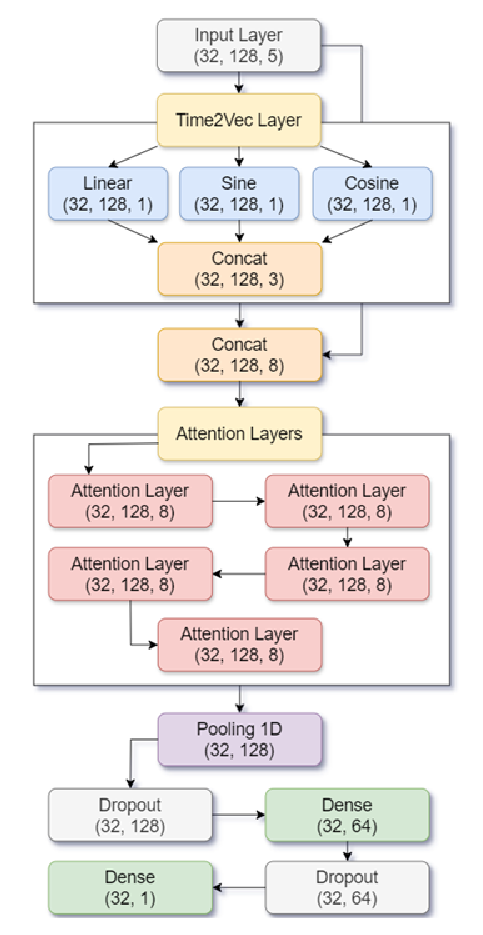
\includegraphics[width=0.6\linewidth]{images/model.eps}
	\caption{Propose model.}
	\label{fig:model}
\end{figure}

Each colored rectangle in the \autoref{fig:model} represents a layer.

Each layer have a tuple of numbers represent the output size after the input
pass through it.
\begin{enumerate}
	\item \textbf{Input Layer}: Take the processed data.
	
	\item \textbf{Time2Vec Layer}: This layer contains 4 sub-layers
	\begin{enumerate}
		\item \textbf{Linear}
		
		- This layer is used for capturing linear trends include steady increase
		and decrease in prices overtime - which might not be periodic but still play
		an important role in time-series.
		
		\item \textbf{Sine} and \textbf{Cosine}
		
		- These two layers are really important for our model. Their first task is
		encoding positions which we can consider as time - represents continuous
		time instead of discrete positions. They also capture the periodic
		behaviors of prices.
		
		- In the Time2Vec paper, they use only one periodic function that is sine
		\autoref{t2v}. But after experiment, we realize that using an additional
		periodic function will yield a better result in this case.
		
		\item \textbf{Concat}
		
		- Use for concatenating above three layers, preparing for next steps.
	\end{enumerate}
	
	\item \textbf{Concat}: This layer take Input layer and combine it with the output
	from Time2Vec layer. We make a residual connections - as known as ResNet
	\cite{resnet}. This action significantly improve the behavior of the network
	which makes the Time2Vec layer more valuable and powerful to our architecture
	and our model.
	
	\item \textbf{Attention Layers}: As known as Multi-head Attention layer, this
	group contains 5 single consecutive attention layers. This structure allow our
	model to jointly attend to values from different aspects at different positions
	ensure that the model can study the trend as clear as possible.
	
	\item \textbf{Pooling 1D}: This layer is responsible for reducing the spatial dimensions
	of the output from Multi-head Attention layers, in terms of width and height,
	while retaining the most important information.
	
	\item \textbf{Dropout}: We need to prevent over-fitting the model. Chosen
	dropout rate is 0.1.
	
	\item \textbf{Dense}: Dense is a fully-connected neural network layer. The first
	Dense applies the activate functions ReLU (see \autoref{relu}) and the other applies
	linear activation function. We use it for decreasing the data dimension.
\end{enumerate}

\section{Why it must be this model?}
We choose Time2Vec to catch continuous attribute of time in the data, the Attention to get a deep understanding of the movement of the trend, the Dropout to prevent over-fitting. We believe that each layer play an important role in the architecture.

\section{Result and Evaluation}
For evaluation, we will split input into 3 parts before actually put them into training
process. Train data will be 80\% of the input. Validation data will be the next
10\% of the input. Test data will be 10\% left of the input.

\subsection{Result of Group 1: NASDAQ, S\&P500, DJI, DAX}
We have trained 5 models for this group.

\textbf{Note}: Multi-feature models are M1\_1, and M1\_4.

\textbf{Note}: One feature models are M1\_2 and M1\_3.

\begin{enumerate}
	\item M1\_1: nas\_sp\_dji\_dax (\autoref{m11})
	
	Features: NASDAQ, S\&P500, DJI, and DAX
	
	\item M1\_2: nas (\autoref{m12})
	
	Features: NASDAQ
	
	\item M1\_3: sp (\autoref{m13})
	
	Features: S\&P500
	
	\item M1\_4: nas\_sp\ (\autoref{m14})
	
	Features: NASDAQ, S\&P500
	
	\begin{table}[H]
		\centering
		\begin{minipage}{0.45\textwidth}
			\centering
			\subcaption[c]{M1\_1}
			\begin{tabular}{|c|c|}
				\hline
				\textbf{Train MAE}  & 0.0127 \\
				\hline
				\textbf{Train MAPE} & 2.3391 \\
				\hline
				\textbf{Train loss} & 0.0004 \\
				\hline
				\textbf{Val MAE}    & 0.0131 \\
				\hline
				\textbf{Val MAPE}   & 2.1929 \\
				\hline
				\textbf{Val loss}   & 0.0004 \\
				\hline
				\textbf{Test MAE}   & 0.0147 \\
				\hline
				\textbf{Test MAPE}  & 3.3804 \\
				\hline
				\textbf{Test loss}  & 0.0006 \\
				\hline
			\end{tabular}
			\label{m11}
		\end{minipage}
		\begin{minipage}{0.45\textwidth}
			\centering
			\subcaption[c]{M1\_2}
			\begin{tabular}{|c|c|}
				\hline
				\textbf{Train MAE}  & 0.0137 \\
				\hline
				\textbf{Train MAPE} & 2.2923 \\
				\hline
				\textbf{Train loss} & 0.0004 \\
				\hline
				\textbf{Val MAE}    & 0.0124 \\
				\hline
				\textbf{Val MAPE}   & 2.0052 \\
				\hline
				\textbf{Val loss}   & 0.0003 \\
				\hline
				\textbf{Test MAE}   & 0.0192 \\
				\hline
				\textbf{Test MAPE}  & 3.2285 \\
				\hline
				\textbf{Test loss}  & 0.0008 \\
				\hline
			\end{tabular}
			\label{m12}
		\end{minipage}
		\begin{minipage}{0.45\textwidth}
			\centering
			\subcaption[c]{M1\_3}
			\begin{tabular}{|c|c|}
				\hline
				\textbf{Train MAE}  & 0.0106 \\
				\hline
				\textbf{Train MAPE} & 2.1629 \\
				\hline
				\textbf{Train loss} & 0.0003 \\
				\hline
				\textbf{Val MAE}    & 0.0119 \\
				\hline
				\textbf{Val MAPE}   & 2.4171 \\
				\hline
				\textbf{Val loss}   & 0.0004 \\
				\hline
				\textbf{Test MAE}   & 0.0108 \\
				\hline
				\textbf{Test MAPE}  & 2.1768 \\
				\hline
				\textbf{Test loss}  & 0.0003 \\
				\hline
			\end{tabular}
			\label{m13}
		\end{minipage}
		\begin{minipage}{0.45\textwidth}
			\centering
			\subcaption[c]{M1\_4}
			\begin{tabular}{|c|c|}
				\hline
				\textbf{Train MAE}  & 0.0105 \\
				\hline
				\textbf{Train MAPE} & 2.0188 \\
				\hline
				\textbf{Train loss} & 0.0003 \\
				\hline
				\textbf{Val MAE}    & 0.0128 \\
				\hline
				\textbf{Val MAPE}   & 2.3027 \\
				\hline
				\textbf{Val loss}   & 0.0004 \\
				\hline
				\textbf{Test MAE}   & 0.0119 \\
				\hline
				\textbf{Test MAPE}  & 2.15   \\
				\hline
				\textbf{Test loss}  & 0.0003 \\
				\hline
			\end{tabular}
			\label{m14}
		\end{minipage}
		\caption{Metrics for models in Group 1}
	\end{table}
\end{enumerate}

\subsection{Evaluation for Group 1}
\label{sub:eval1} 

We can see that M1\_4 (\autoref{m14}) yields better result than M1\_1 (\autoref{m11}) which means
that 4 features does not lead to a better model.

We can also point out that M1\_4 (\autoref{m14}) have better results than
M1\_2 (\autoref{m12}) and M1\_3 (\autoref{m13}). This means that the multi-feature models
\textbf{may} work better than the single-feature models.

\subsection{Result of Group 2: Exxon Mobil, Chervon}
We have trained 3 models for this group.

\textbf{Note}: Multi-feature model is M2\_3.

\textbf{Note}: One feature models are M2\_1 and M2\_2.


\begin{enumerate}
	\item M2\_1: exxon (\autoref{m21})
	
	Features: Exxon
	
	\item M2\_2: chervon (\autoref{m22})
	
	Features: Chervon
	
	\item M2\_3: exxon\_chervon (\autoref{m23})
	
	Features: Exxon, Chervon
	
	\begin{table}[H]
		\centering
		\begin{minipage}{0.3\textwidth}
			\centering
			\subcaption[c]{M2\_1}
			\begin{tabular}{|c|c|}
				\hline
				\textbf{Train MAE}  & 0.0138 \\
				\hline
				\textbf{Train MAPE} & 2.1378 \\
				\hline
				\textbf{Train loss} & 0.0003 \\
				\hline
				\textbf{Val MAE}    & 0.012  \\
				\hline
				\textbf{Val MAPE}   & 1.8924 \\
				\hline
				\textbf{Val loss}   & 0.0003 \\
				\hline
				\textbf{Test MAE}   & 0.0303 \\
				\hline
				\textbf{Test MAPE}  & 6.14   \\
				\hline
				\textbf{Test loss}  & 0.0028 \\
				\hline
			\end{tabular}
			\label{m21}
		\end{minipage}
		\begin{minipage}{0.3\textwidth}
			\centering
			\subcaption[c]{M2\_2}
			\begin{tabular}{|c|c|}
				\hline
				\textbf{Train MAE}  & 0.0114 \\
				\hline
				\textbf{Train MAPE} & 1.9157 \\
				\hline
				\textbf{Train loss} & 0.0002 \\
				\hline
				\textbf{Val MAE}    & 0.0099 \\
				\hline
				\textbf{Val MAPE}   & 1.6689 \\
				\hline
				\textbf{Val loss}   & 0.0002 \\
				\hline
				\textbf{Test MAE}   & 0.0163 \\
				\hline
				\textbf{Test MAPE}  & 3.7077 \\
				\hline
				\textbf{Test loss}  & 0.0009 \\
				\hline
			\end{tabular}
			\label{m22}
		\end{minipage}
		\begin{minipage}{0.3\textwidth}
			\centering
			\subcaption[c]{M2\_3}
			\begin{tabular}{|c|c|}
				\hline
				\textbf{Train MAE}  & 0.011  \\
				\hline
				\textbf{Train MAPE} & 1.7753 \\
				\hline
				\textbf{Train loss} & 0.0002 \\
				\hline
				\textbf{Val MAE}    & 0.0096 \\
				\hline
				\textbf{Val MAPE}   & 1.5592 \\
				\hline
				\textbf{Val loss}   & 0.0002 \\
				\hline
				\textbf{Test MAE}   & 0.018  \\
				\hline
				\textbf{Test MAPE}  & 3.8575 \\
				\hline
				\textbf{Test loss}  & 0.0011 \\
				\hline
			\end{tabular}
			\label{m23}
		\end{minipage}
		\caption{Metrics for models in Group 2}
	\end{table}
\end{enumerate}

\subsection{Evaluation for Group 2}
The results in \autoref{sub:eval1} show similar findings here.

Multi-feature models outperform single-feature model, as evidenced by M2\_3 (\autoref{m23})
being superior to M2\_1 (\autoref{m21}). However, model M2\_2 slightly outperforms the multi-feature models, as indicated in \autoref{m22}.

This shows that although multi-feature model outperforms one-feature models under certain circumstances, special one-feature model may still have better performance.

\section{Further evaluation}
From now on, we will not split the data into 3 parts (train, validation, and test) to evaluate since we have the models (as trained above).

Moreover, we will use RMSE (from \autoref{rmse}), MSE (from \autoref{mse}), and R2
(from \autoref{r2}) as additional metrics with MAPE (from \autoref{mape}) and MAE
(from \autoref{mae}) to have a clearly evaluation for models.

We also use Accuracy, Precision (Pre), Recall, and F1-score (F1) to evaluate our
trend prediction (classification problem).

\textbf{Note}: Accuracy, Pre, Recall, F1-score will evaluate on 2 labels:
Decreasing, and Non-decreasing. We will se there is only one value for Accuracy
but two for the others (the left value will be for label 0, the right value will
be for label1).

\subsection{Method for decoding predicted output to prices}
We need to follow the pipeline how we pre-processed the data to decode it.
\autoref{fig:decode} describes the decoding pipeline.
\begin{figure}[H]
	\centering
	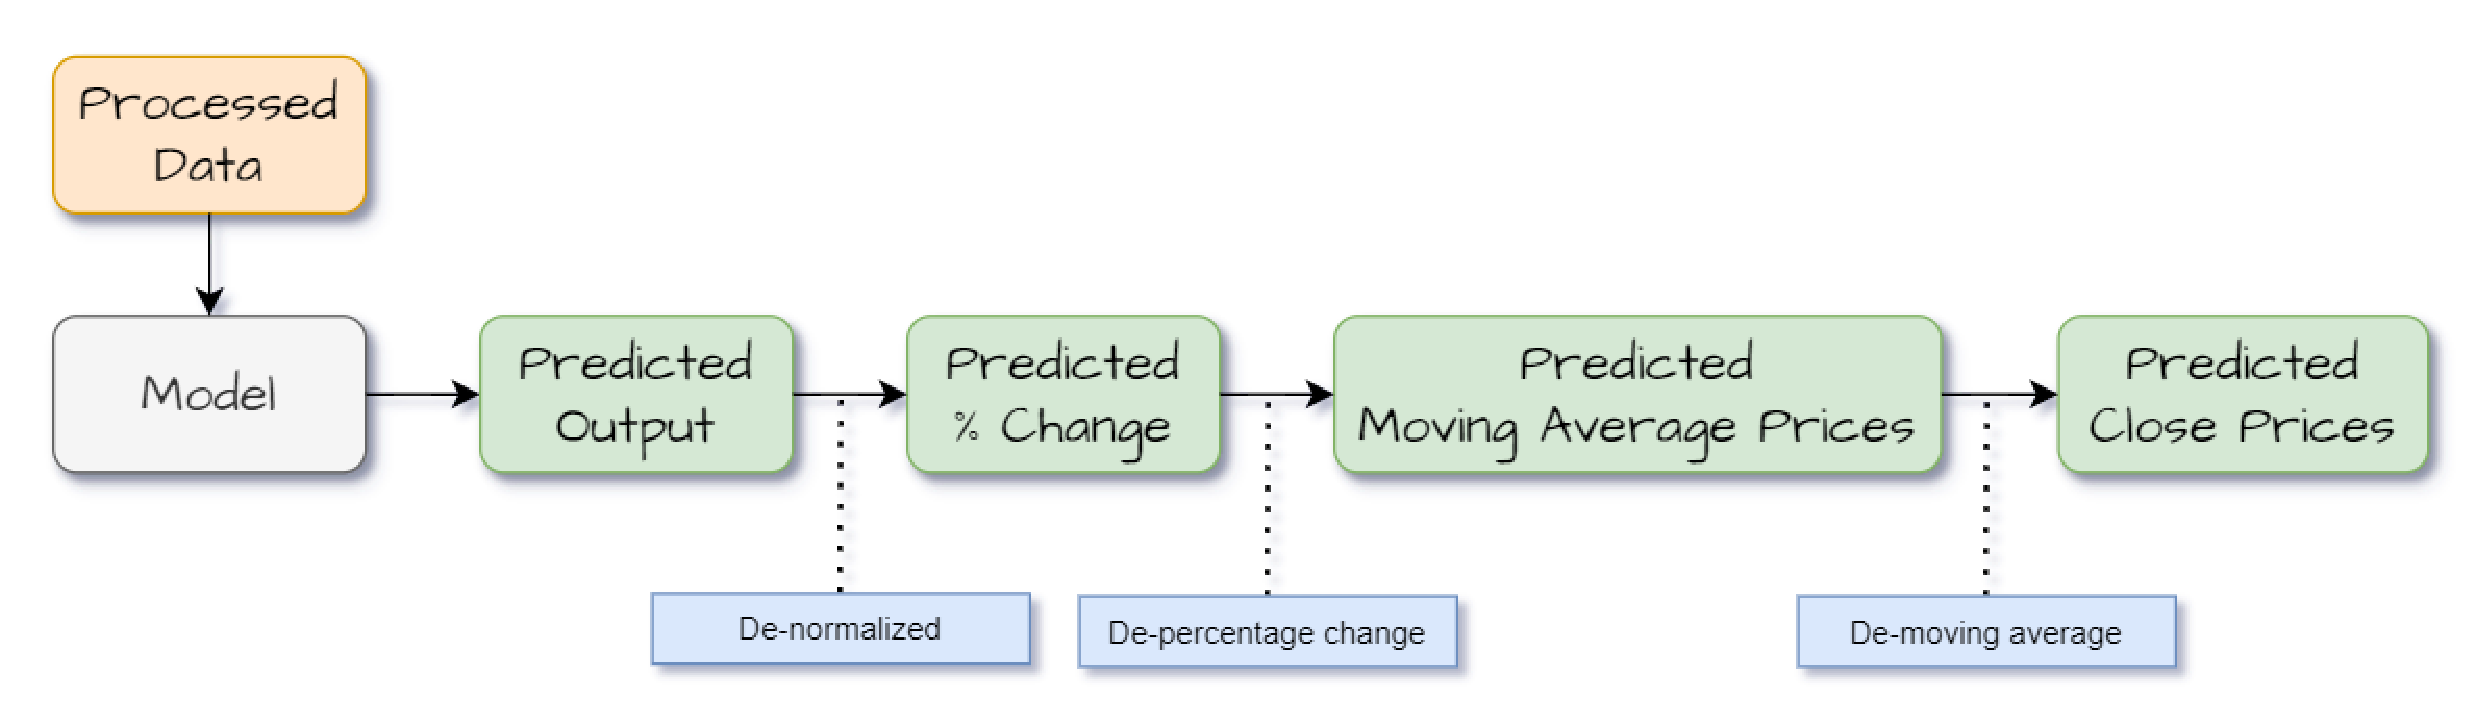
\includegraphics[width=1\linewidth]{images/decode.eps}
	\caption{Decode predicted output pipeline.}
	\label{fig:decode}
\end{figure}
Walk-through for each step in the pipeline.

\textbf{Note that}: $x$ is used for predicted values, $v$ is use for real values.
\begin{enumerate}
	\item \textbf{De-normalized step}: This step include 2 small steps in it.
	\begin{enumerate}
		\item Making sure that the output is between 0 and 1, if there exist
		values such that $x_{i}>1$ we will take its reciprocal instead. Cases that
		$x_{i}< 0$ seem to not occur in experiment.
		
		\item Apply min-max de-normalized formula:
		\begin{equation}
			x_{pct}=x_{nor}\times(max-min)+min \label{de-nor}
		\end{equation}
		$x_{predict nor}$: vector of output from model (predicted normalized
		values).
		
		$max$, $min$: max and min value from \autoref{normalized}.
		
		$x_{pct}$: vector of predicted percentage change values.
		
		\textbf{Note that}: $max$ and $min$ is max and min of open, high, low, and
		close.
	\end{enumerate}
	
	\item \textbf{De-percentage change step}:
	\begin{equation}
		x_{mva}=\left\{
		\begin{array}{l}
			v_{pct}, i=0                                    \\
			v_{pct} \times\left(1+x_{pct}\right), otherwise
		\end{array}\right. \label{de-pct}
	\end{equation}
	$v_{pct}$: vector of real percentage change values.
	
	$x_{pct}$: vector of predicted percentage change values.
	
	$v_{mva}$: vector of predicted moving average prices.
	
	\item \textbf{De-moving average step}:
	\begin{equation}
		x_{close}=
		\begin{cases}
			v_{close}       & , i \leq s-1                            \\
			x_{mva}\times s & - \sum_{k=i-s}^{i-1}v_{close}, i \geq s
		\end{cases}
		\label{de-moving}
	\end{equation}
	$x_{mva}$: vector of predicted moving average prices.
	
	$v_{close}$: vector of real close prices.
	
	$x_{close}$: vector of predicted close prices.
	
	$s$: moving average step
	
	\bigskip
	
	In this thesis, we follow moving average strategy every fortnight which
	means our step will be 14. So that, \autoref{de-moving} can also be written as
	\begin{equation}
		x_{close}=
		\begin{cases}
			v_{close}        & , i \leq 13                               \\
			x_{mva}\times 14 & - \sum_{k=i-14}^{i-1}v_{close}, i \geq 14
		\end{cases}
	\end{equation}
\end{enumerate}

\subsection{Deep evaluation with respect to NASDAQ}
In terms of NASDAQ, we can use M1\_1, M1\_2, and M1\_4. These model contains NASDAQ as a feature in them.

\begin{table}[H]
	\centering
	\begin{minipage}{0.3\textwidth}
		\centering
		\subcaption[c]{M1\_1}
		\begin{tabular}{|c|c|}
			\hline
			\textbf{RMSE} & 0.025553224 \\
			\hline
			\textbf{MSE}  & 0.000652967 \\
			\hline
			\textbf{MAPE} & 2.83452573  \\
			\hline
			\textbf{MAE}  & 0.016752568 \\
			\hline
			\textbf{R2}   & 0.836478961 \\
			\hline
		\end{tabular}
	\end{minipage}
	\begin{minipage}{0.3\textwidth}
		\centering
		\subcaption[c]{M1\_2}
		\begin{tabular}{|c|c|}
			\hline
			\textbf{RMSE} & 0.01870842  \\
			\hline
			\textbf{MSE}  & 0.000350005 \\
			\hline
			\textbf{MAPE} & 2.006188642 \\
			\hline
			\textbf{MAE}  & 0.011983401 \\
			\hline
			\textbf{R2}   & 0.91235242  \\
			\hline
		\end{tabular}
	\end{minipage}
	\begin{minipage}{0.3\textwidth}
		\centering
		\subcaption[c]{M1\_4}
		\begin{tabular}{|c|c|}
			\hline
			\textbf{RMSE} & 0.02125059  \\
			\hline
			\textbf{MSE}  & 0.000451588 \\
			\hline
			\textbf{MAPE} & 2.408059498 \\
			\hline
			\textbf{MAE}  & 0.014652739 \\
			\hline
			\textbf{R2}   & 0.886914298 \\
			\hline
		\end{tabular}
	\end{minipage}
	\caption{Predicting normalized values metrics of the NASDAQ dataset.}
	\label{metric:nasdaq_nor}
\end{table}
\begin{table}[H]
	\centering
	\begin{minipage}{0.3\textwidth}
		\centering
		\subcaption[c]{M1\_1}
		\begin{tabular}{|c|c|}
			\hline
			\textbf{RMSE} & 5.73749947  \\
			\hline
			\textbf{MSE}  & 32.91890017 \\
			\hline
			\textbf{MAPE} & 0.076206824 \\
			\hline
			\textbf{MAE}  & 2.399314816 \\
			\hline
			\textbf{R2}   & 0.999997427 \\
			\hline
		\end{tabular}
	\end{minipage}
	\begin{minipage}{0.3\textwidth}
		\centering
		\subcaption[c]{M1\_2}
		\begin{tabular}{|c|c|}
			\hline
			\textbf{RMSE} & 4.56276691  \\
			\hline
			\textbf{MSE}  & 20.81884188 \\
			\hline
			\textbf{MAPE} & 0.054502324 \\
			\hline
			\textbf{MAE}  & 1.727510579 \\
			\hline
			\textbf{R2}   & 0.999998373 \\
			\hline
		\end{tabular}
	\end{minipage}
	\begin{minipage}{0.3\textwidth}
		\centering
		\subcaption[c]{M1\_4}
		\begin{tabular}{|c|c|}
			\hline
			\textbf{RMSE} & 4.774897561 \\
			\hline
			\textbf{MSE}  & 22.79964672 \\
			\hline
			\textbf{MAPE} & 0.066603007 \\
			\hline
			\textbf{MAE}  & 2.009664443 \\
			\hline
			\textbf{R2}   & 0.999998218 \\
			\hline
		\end{tabular}
	\end{minipage}
	\caption{Predicting moving average values of the NASDAQ dataset.}
	\label{metric:nasdaq_mva}
\end{table}
\begin{table}[H]
	\centering
	\begin{minipage}{0.3\textwidth}
		\centering
		\subcaption[c]{M1\_1}
		\begin{tabular}{|c|c|}
			\hline
			\textbf{RMSE} & 80.29814013 \\
			\hline
			\textbf{MSE}  & 6447.791308 \\
			\hline
			\textbf{MAPE} & 1.069284617 \\
			\hline
			\textbf{MAE}  & 33.56795279 \\
			\hline
			\textbf{R2}   & 0.999498387 \\
			\hline
		\end{tabular}
	\end{minipage}
	\begin{minipage}{0.3\textwidth}
		\centering
		\subcaption[c]{M1\_2}
		\begin{tabular}{|c|c|}
			\hline
			\textbf{RMSE} & 63.85738223 \\
			\hline
			\textbf{MSE}  & 4077.765265 \\
			\hline
			\textbf{MAPE} & 0.764418767 \\
			\hline
			\textbf{MAE}  & 24.16898073 \\
			\hline
			\textbf{R2}   & 0.999682766 \\
			\hline
		\end{tabular}
	\end{minipage}
	\begin{minipage}{0.3\textwidth}
		\centering
		\subcaption[c]{M1\_4}
		\begin{tabular}{|c|c|}
			\hline
			\textbf{RMSE} & 66.82621854 \\
			\hline
			\textbf{MSE}  & 4465.743484 \\
			\hline
			\textbf{MAPE} & 0.929676058 \\
			\hline
			\textbf{MAE}  & 28.11649422 \\
			\hline
			\textbf{R2}   & 0.999652583 \\
			\hline
		\end{tabular}
	\end{minipage}
	\caption{Predicting close price metrics of the NASDAQ dataset.}
	\label{metric:nasdaq_close}
\end{table}
\begin{table}[H]
	\centering
	\begin{minipage}{0.45\textwidth}
		\centering
		\subcaption[c]{M1\_1}
		\begin{tabular}{|c|c|c|}
			\hline
			\textbf{Acc}    & \multicolumn{2}{c|}{0.8921} \\
			\hline
			\textbf{Pre}    & 0.85623003                 & 0.91801682 \\
			\hline
			\textbf{Recall} & 0.88347914                 & 0.89922817 \\
			\hline
			\textbf{F1}     & 0.86964119                 & 0.90852537 \\
			\hline
		\end{tabular}
	\end{minipage}
	\begin{minipage}{0.45\textwidth}
		\centering
		\subcaption[c]{M1\_2}
		\begin{tabular}{|c|c|c|}
			\hline
			\textbf{Acc}    & \multicolumn{2}{c|}{0.9026} \\
			\hline
			\textbf{Pre}    & 0.87157555                 & 0.92468766 \\
			\hline
			\textbf{Recall} & 0.89146697                 & 0.91027196 \\
			\hline
			\textbf{F1}     & 0.88140905                 & 0.91742318 \\
			\hline
		\end{tabular}
	\end{minipage}
	\begin{minipage}{0.45\textwidth}
		\centering
		\subcaption[c]{M1\_4}
		\begin{tabular}{|c|c|c|}
			\hline
			\textbf{Acc}    & \multicolumn{2}{c|}{0.912} \\
			\hline
			\textbf{Pre}    & 0.89040576                & 0.92683562 \\
			\hline
			\textbf{Recall} & 0.89311525                & 0.92490906 \\
			\hline
			\textbf{F1}     & 0.89175845                & 0.92587134 \\
			\hline
		\end{tabular}
	\end{minipage}
	\caption{Predicting trend metrics of the NASDAQ dataset.}
	\label{metric:nasdaq_trend}
\end{table}

Base on \autoref{metric:nasdaq_nor}, \autoref{metric:nasdaq_mva}, \autoref{metric:nasdaq_close},
and \autoref{metric:nasdaq_trend}. We can proudly say that, with respect to
NASDAQ, model M1\_2 (one-feature) and model M1\_4 (two-feature) outperform model M1\_1 (four-feature).

In terms of comparing between M1\_2 and M1\_4, we can say that the multi-feature
one (M1\_5) is better in the real world - when people usually look for the trend
of a stock rather than at its real prices.

However, both play very good predictions, their trade-offs are tiny, so that we can
pick any of them to use.

\subsection{Deep evaluation with respect to S\&P500}
In terms of S\&P500, we can use M1\_1, M1\_3, M1\_4. These model contains
S\&P500 as a feature in them.

\begin{table}[H]
	\centering
	\begin{minipage}{0.3\textwidth}
		\centering
		\subcaption[c]{M1\_1}
		\begin{tabular}{|c|c|}
			\hline
			\textbf{RMSE} & 0.018034203 \\
			\hline
			\textbf{MSE}  & 0.000325232 \\
			\hline
			\textbf{MAPE} & 2.242464144 \\
			\hline
			\textbf{MAE}  & 0.011113481 \\
			\hline
			\textbf{R2}   & 0.883783973 \\
			\hline
		\end{tabular}
	\end{minipage}
	\begin{minipage}{0.3\textwidth}
		\centering
		\subcaption[c]{M1\_3}
		\begin{tabular}{|c|c|}
			\hline
			\textbf{RMSE} & 0.017224297 \\
			\hline
			\textbf{MSE}  & 0.000296676 \\
			\hline
			\textbf{MAPE} & 2.208480955 \\
			\hline
			\textbf{MAE}  & 0.01112233  \\
			\hline
			\textbf{R2}   & 0.893987027 \\
			\hline
		\end{tabular}
	\end{minipage}
	\begin{minipage}{0.3\textwidth}
		\centering
		\subcaption[c]{M1\_4}
		\begin{tabular}{|c|c|}
			\hline
			\textbf{RMSE} & 0.016504522 \\
			\hline
			\textbf{MSE}  & 0.000272399 \\
			\hline
			\textbf{MAPE} & 1.960718136 \\
			\hline
			\textbf{MAE}  & 0.009845696 \\
			\hline
			\textbf{R2}   & 0.902662108 \\
			\hline
		\end{tabular}
	\end{minipage}
	\caption{Predicting normalized values metrics of the S\&P500 dataset.}
	\label{metric:sp_nor}
\end{table}
\begin{table}[H]
	\centering
	\begin{minipage}{0.3\textwidth}
		\centering
		\subcaption[c]{M1\_1}
		\begin{tabular}{|c|c|}
			\hline
			\textbf{RMSE} & 1.020056917 \\
			\hline
			\textbf{MSE}  & 1.040516114 \\
			\hline
			\textbf{MAPE} & 0.055009158 \\
			\hline
			\textbf{MAE}  & 0.34066933  \\
			\hline
			\textbf{R2}   & 0.99999897  \\
			\hline
		\end{tabular}
	\end{minipage}
	\begin{minipage}{0.3\textwidth}
		\centering
		\subcaption[c]{M1\_3}
		\begin{tabular}{|c|c|}
			\hline
			\textbf{RMSE} & 1.016457032 \\
			\hline
			\textbf{MSE}  & 1.033184897 \\
			\hline
			\textbf{MAPE} & 0.055034722 \\
			\hline
			\textbf{MAE}  & 0.347453224 \\
			\hline
			\textbf{R2}   & 0.999998977 \\
			\hline
		\end{tabular}
	\end{minipage}
	\begin{minipage}{0.3\textwidth}
		\centering
		\subcaption[c]{M1\_4}
		\begin{tabular}{|c|c|}
			\hline
			\textbf{RMSE} & 0.922520875 \\
			\hline
			\textbf{MSE}  & 0.851044764 \\
			\hline
			\textbf{MAPE} & 0.048713757 \\
			\hline
			\textbf{MAE}  & 0.303149401 \\
			\hline
			\textbf{R2}   & 0.999999157 \\
			\hline
		\end{tabular}
	\end{minipage}
	\caption{Predicting moving average values metrics of the S\&P500 dataset.}
	\label{metric:sp_mva}
\end{table}
\begin{table}[H]
	\centering
	\begin{minipage}{0.3\textwidth}
		\centering
		\subcaption[c]{M1\_1}
		\begin{tabular}{|c|c|}
			\hline
			\textbf{RMSE} & 14.27815877 \\
			\hline
			\textbf{MSE}  & 203.8658177 \\
			\hline
			\textbf{MAPE} & 0.773167971 \\
			\hline
			\textbf{MAE}  & 4.767608709 \\
			\hline
			\textbf{R2}   & 0.999798843 \\
			\hline
		\end{tabular}
	\end{minipage}
	\begin{minipage}{0.3\textwidth}
		\centering
		\subcaption[c]{M1\_3}
		\begin{tabular}{|c|c|}
			\hline
			\textbf{RMSE} & 14.22776968 \\
			\hline
			\textbf{MSE}  & 202.4294301 \\
			\hline
			\textbf{MAPE} & 0.771584123 \\
			\hline
			\textbf{MAE}  & 4.86254813  \\
			\hline
			\textbf{R2}   & 0.99980026  \\
			\hline
		\end{tabular}
	\end{minipage}
	\begin{minipage}{0.3\textwidth}
		\centering
		\subcaption[c]{M1\_4}
		\begin{tabular}{|c|c|}
			\hline
			\textbf{RMSE} & 12.91290642 \\
			\hline
			\textbf{MSE}  & 166.7431522 \\
			\hline
			\textbf{MAPE} & 0.683400608 \\
			\hline
			\textbf{MAE}  & 4.242523745 \\
			\hline
			\textbf{R2}   & 0.999835472 \\
			\hline
		\end{tabular}
	\end{minipage}
	\caption{Predicting close price metrics of the S\&P500 dataset.}
	\label{metric:sp_close}
\end{table}
\begin{table}[H]
	\centering
	\begin{minipage}{0.45\textwidth}
		\centering
		\subcaption[c]{M1\_1}
		\begin{tabular}{|c|c|c|}
			\hline
			\textbf{Acc}    & \multicolumn{2}{c|}{0.8911} \\
			\hline
			\textbf{Pre}    & 0.86583744                 & 0.90993943 \\
			\hline
			\textbf{Recall} & 0.88077678                 & 0.90356932 \\
			\hline
			\textbf{F1}     & 0.87324322                 & 0.90674319 \\
			\hline
		\end{tabular}
	\end{minipage}
	\begin{minipage}{0.45\textwidth}
		\centering
		\subcaption[c]{M1\_3}
		\begin{tabular}{|c|c|c|}
			\hline
			\textbf{Acc}    & \multicolumn{2}{c|}{0.8914} \\
			\hline
			\textbf{Pre}    & 0.86586099                 & 0.9103421  \\
			\hline
			\textbf{Recall} & 0.87746126                 & 0.90150512 \\
			\hline
			\textbf{F1}     & 0.87162253                 & 0.90590206 \\
			\hline
		\end{tabular}
	\end{minipage}
	\begin{minipage}{0.45\textwidth}
		\centering
		\subcaption[c]{M1\_4}
		\begin{tabular}{|c|c|c|}
			\hline
			\textbf{Acc}    & \multicolumn{2}{c|}{0.8975} \\
			\hline
			\textbf{Pre}    & 0.87868519                 & 0.91116987 \\
			\hline
			\textbf{Recall} & 0.87725827                 & 0.912242   \\
			\hline
			\textbf{F1}     & 0.87797115                 & 0.91170562 \\
			\hline
		\end{tabular}
	\end{minipage}
	\caption{Predicting trend metrics of the S\&P500 dataset.}
	\label{metric:sp_trend}
\end{table}

Base on \autoref{metric:sp_nor}, \autoref{metric:sp_mva},
\autoref{metric:sp_close}, and \autoref{metric:sp_trend}. We can proudly say
that, with respect to S\&P500, model M1\_5 outperform the others.

\subsection{Deep evaluation with respect to Exxon Mobil}
In terms of Exxon Mobil, we can use M2\_1 and M2\_3. These model contains
Exxon Mobil as a feature in them.

\begin{table}[H]
	\centering
	\begin{minipage}{0.45\textwidth}
		\centering
		\subcaption[c]{M2\_1}
		\begin{tabular}{|c|c|}
			\hline
			\textbf{RMSE} & 0.023179541 \\
			\hline
			\textbf{MSE}  & 0.000537291 \\
			\hline
			\textbf{MAPE} & 2.290878355 \\
			\hline
			\textbf{MAE}  & 0.013910819 \\
			\hline
			\textbf{R2}   & 0.801418014 \\
			\hline
		\end{tabular}
	\end{minipage}
	\begin{minipage}{0.45\textwidth}
		\centering
		\subcaption[c]{M2\_3}
		\begin{tabular}{|c|c|}
			\hline
			\textbf{RMSE} & 0.02010469  \\
			\hline
			\textbf{MSE}  & 0.000404199 \\
			\hline
			\textbf{MAPE} & 2.158960848 \\
			\hline
			\textbf{MAE}  & 0.01338959  \\
			\hline
			\textbf{R2}   & 0.85060855  \\
			\hline
		\end{tabular}
	\end{minipage}
	\caption{Predicting normalized values metrics of the Exxon dataset.}
	\label{metric:exx_nor}
\end{table}
\begin{table}[H]
	\centering
	\begin{minipage}{0.45\textwidth}
		\centering
		\subcaption[c]{M2\_1}
		\begin{tabular}{|c|c|}
			\hline
			\textbf{RMSE} & 0.048242004 \\
			\hline
			\textbf{MSE}  & 0.002327291 \\
			\hline
			\textbf{MAPE} & 0.075914309 \\
			\hline
			\textbf{MAE}  & 0.01831591  \\
			\hline
			\textbf{R2}   & 0.999996625 \\
			\hline
		\end{tabular}
	\end{minipage}
	\begin{minipage}{0.45\textwidth}
		\centering
		\subcaption[c]{M2\_3}
		\begin{tabular}{|c|c|}
			\hline
			\textbf{RMSE} & 0.03920276  \\
			\hline
			\textbf{MSE}  & 0.001536856 \\
			\hline
			\textbf{MAPE} & 0.073085054 \\
			\hline
			\textbf{MAE}  & 0.016113275 \\
			\hline
			\textbf{R2}   & 0.999997771 \\
			\hline
		\end{tabular}
	\end{minipage}
	\caption{Predicting moving average values metrics of the Exxon dataset.}
	\label{metric:exx_mva}
\end{table}
\begin{table}[H]
	\centering
	\begin{minipage}{0.45\textwidth}
		\centering
		\subcaption[c]{M2\_1}
		\begin{tabular}{|c|c|}
			\hline
			\textbf{RMSE} & 0.675197252 \\
			\hline
			\textbf{MSE}  & 0.455891329 \\
			\hline
			\textbf{MAPE} & 1.061601097 \\
			\hline
			\textbf{MAE}  & 0.256277127 \\
			\hline
			\textbf{R2}   & 0.999341621 \\
			\hline
		\end{tabular}
	\end{minipage}
	\begin{minipage}{0.45\textwidth}
		\centering
		\subcaption[c]{M2\_3}
		\begin{tabular}{|c|c|}
			\hline
			\textbf{RMSE} & 0.548681928 \\
			\hline
			\textbf{MSE}  & 0.301051858 \\
			\hline
			\textbf{MAPE} & 1.020793064 \\
			\hline
			\textbf{MAE}  & 0.225457042 \\
			\hline
			\textbf{R2}   & 0.999565233 \\
			\hline
		\end{tabular}
	\end{minipage}
	\caption{Predicting close price metrics of the Exxon dataset.}
	\label{metric:exx_close}
\end{table}
\begin{table}[H]
	\centering
	\begin{minipage}{0.45\textwidth}
		\centering
		\subcaption[c]{M2\_1}
		\begin{tabular}{|c|c|c|}
			\hline
			\textbf{Acc}    & \multicolumn{2}{c|}{0.8794} \\
			\hline
			\textbf{Pre}    & 0.85236517                 & 0.90044542 \\
			\hline
			\textbf{Recall} & 0.86948059                 & 0.88686216 \\
			\hline
			\textbf{F1}     & 0.86083781                 & 0.89360217 \\
			\hline
		\end{tabular}
	\end{minipage}
	\begin{minipage}{0.45\textwidth}
		\centering
		\subcaption[c]{M2\_3}
		\begin{tabular}{|c|c|c|}
			\hline
			\textbf{Acc}    & \multicolumn{2}{c|}{0.8746} \\
			\hline
			\textbf{Pre}    & 0.84454201                 & 0.89820924 \\
			\hline
			\textbf{Recall} & 0.86721311                 & 0.88009851 \\
			\hline
			\textbf{F1}     & 0.85572743                 & 0.88906165 \\
			\hline
		\end{tabular}
	\end{minipage}
	\caption{Predicting trend metrics of the Exxon dataset.}
	\label{metric:exx_trend}
\end{table}

Base on \autoref{metric:exx_nor}, \autoref{metric:exx_mva},
\autoref{metric:exx_close}, and \autoref{metric:exx_trend}. We can proudly say
that, with respect to Exxon Mobil, model M2\_3 outperform the other one. Despite the
fact that M2\_1 has a slightly better in predicting trend, the difference
between M2\_1 and M2\_3 in that area is less than 1\% which is not considerable.
So that our multi-feature model work well in this case.

\subsection{Deep evaluation with respect to Chervon}
In terms of Chervon, we can use M2\_2 and M2\_3. These model contains Chervon as a feature in them.

\begin{table}[H]
	\centering
	\begin{minipage}{0.45\textwidth}
		\centering
		\subcaption[c]{M2\_2}
		\begin{tabular}{|c|c|}
			\hline
			\textbf{RMSE} & 0.01682611  \\
			\hline
			\textbf{MSE}  & 0.000283118 \\
			\hline
			\textbf{MAPE} & 1.929007573 \\
			\hline
			\textbf{MAE}  & 0.010853351 \\
			\hline
			\textbf{R2}   & 0.887236384 \\
			\hline
		\end{tabular}
	\end{minipage}
	\begin{minipage}{0.45\textwidth}
		\centering
		\subcaption[c]{M2\_3}
		\begin{tabular}{|c|c|}
			\hline
			\textbf{RMSE} & 0.017909977 \\
			\hline
			\textbf{MSE}  & 0.000320767 \\
			\hline
			\textbf{MAPE} & 2.090819573 \\
			\hline
			\textbf{MAE}  & 0.011799609 \\
			\hline
			\textbf{R2}   & 0.872240963 \\
			\hline
		\end{tabular}
	\end{minipage}
	\caption{Predicting normalized values metrics of the Chervon dataset.}
	\label{metric:che_nor}
\end{table}
\begin{table}[H]
	\centering
	\begin{minipage}{0.45\textwidth}
		\centering
		\subcaption[c]{M2\_2}
		\begin{tabular}{|c|c|}
			\hline
			\textbf{RMSE} & 0.062136657 \\
			\hline
			\textbf{MSE}  & 0.003860964 \\
			\hline
			\textbf{MAPE} & 0.073510284 \\
			\hline
			\textbf{MAE}  & 0.021515203 \\
			\hline
			\textbf{R2}   & 0.999997359 \\
			\hline
		\end{tabular}
	\end{minipage}
	\begin{minipage}{0.45\textwidth}
		\centering
		\subcaption[c]{M2\_3}
		\begin{tabular}{|c|c|}
			\hline
			\textbf{RMSE} & 0.061813397 \\
			\hline
			\textbf{MSE}  & 0.003820896 \\
			\hline
			\textbf{MAPE} & 0.07992873  \\
			\hline
			\textbf{MAE}  & 0.022514326 \\
			\hline
			\textbf{R2}   & 0.999997386 \\
			\hline
		\end{tabular}
	\end{minipage}
	\caption{Predicting moving average values metrics of the Chervon dataset.}
	\label{metric:che_mva}
\end{table}
\begin{table}[H]
	\centering
	\begin{minipage}{0.45\textwidth}
		\centering
		\subcaption[c]{M2\_2}
		\begin{tabular}{|c|c|}
			\hline
			\textbf{RMSE} & 0.869664813 \\
			\hline
			\textbf{MSE}  & 0.756316888 \\
			\hline
			\textbf{MAPE} & 1.031343171 \\
			\hline
			\textbf{MAE}  & 0.301040856 \\
			\hline
			\textbf{R2}   & 0.999484581 \\
			\hline
		\end{tabular}
	\end{minipage}
	\begin{minipage}{0.45\textwidth}
		\centering
		\subcaption[c]{M2\_3}
		\begin{tabular}{|c|c|}
			\hline
			\textbf{RMSE} & 0.865140471 \\
			\hline
			\textbf{MSE}  & 0.748468035 \\
			\hline
			\textbf{MAPE} & 1.123356882 \\
			\hline
			\textbf{MAE}  & 0.315020592 \\
			\hline
			\textbf{R2}   & 0.99948993  \\
			\hline
		\end{tabular}
	\end{minipage}
	\caption{Predicting close price metrics of the Chervon dataset.}
	\label{metric:che_close}
\end{table}
\begin{table}[H]
	\centering
	\begin{minipage}{0.45\textwidth}
		\centering
		\subcaption[c]{M2\_2}
		\begin{tabular}{|c|c|c|}
			\hline
			\textbf{Acc}    & \multicolumn{2}{c|}{0.8841} \\
			\hline
			\textbf{Pre}    & 0.85960136                 & 0.90432272 \\
			\hline
			\textbf{Recall} & 0.88110425                 & 0.88647799 \\
			\hline
			\textbf{F1}     & 0.87021999                 & 0.89531145 \\
			\hline
		\end{tabular}
	\end{minipage}
	\begin{minipage}{0.45\textwidth}
		\centering
		\subcaption[c]{M2\_3}
		\begin{tabular}{|c|c|c|}
			\hline
			\textbf{Acc}    & \multicolumn{2}{c|}{0.8798} \\
			\hline
			\textbf{Pre}    & 0.85623658                 & 0.89910457 \\
			\hline
			\textbf{Recall} & 0.87424016                 & 0.88418901 \\
			\hline
			\textbf{F1}     & 0.86514472                 & 0.89158441 \\
			\hline
		\end{tabular}
	\end{minipage}
	\caption{Predicting trend metrics of the Chervon dataset.}
	\label{metric:che_trend}
\end{table}
Base on \autoref{metric:che_nor}, \autoref{metric:che_mva}, \autoref{metric:che_close},
and \autoref{metric:che_trend}. We can proudly say that, with respect to Chervon,
M2\_2 and M2\_3 only has a little bit better in total, our multi-feature model is less than the other one at most about 1\% - that is not significant in real life problems.

\section{Comparing to SOTA models}
We will follow all the pre-processing steps before putting the data into LSTM model
and RNN model as well as follow all the decoding steps to have the most fair competition
between models.

\subsection{With respect to NASDAQ}
\begin{table}[H]
	\centering
	\begin{minipage}{0.4\textwidth}
		\centering
		\subcaption[c]{LSTM}
		\begin{tabular}{|c|c|}
			\hline
			\textbf{RMSE} & 0.022196892 \\
			\hline
			\textbf{MSE}  & 0.000492702 \\
			\hline
			\textbf{MAPE} & 2.385642716 \\
			\hline
			\textbf{MAE}  & 0.014343534 \\
			\hline
			\textbf{R2}   & 0.876628911 \\
			\hline
		\end{tabular}
	\end{minipage}
	\begin{minipage}{0.4\textwidth}
		\centering
		\subcaption[c]{RNN}
		\begin{tabular}{|c|c|}
			\hline
			\textbf{RMSE} & 0.047336384
			 \\
			\hline
			\textbf{MSE}  & 0.002240733
			 \\
			\hline
			\textbf{MAPE} & 6.698210951
			 \\
			\hline
			\textbf{MAE}  & 0.041594085
			 \\
			\hline
			\textbf{R2}   & 0.438909067
			 \\
			\hline
		\end{tabular}
	\end{minipage}
	\caption{Predicting normalized values metrics of the NASDAQ dataset.}
	\label{nas:lstm_rnn_nor}
\end{table}
\begin{table}[H]
	\centering
	\begin{minipage}{0.4\textwidth}
		\centering
		\subcaption[c]{LSTM}
		\begin{tabular}{|c|c|}
			\hline
			\textbf{RMSE} & 5.125561613 \\
			\hline
			\textbf{MSE}  & 26.27138185 \\
			\hline
			\textbf{MAPE} & 0.065215182 \\
			\hline
			\textbf{MAE}  & 2.026053739 \\
			\hline
			\textbf{R2}   & 0.999997954 \\
			\hline
		\end{tabular}
	\end{minipage}
	\begin{minipage}{0.4\textwidth}
		\centering
		\subcaption[c]{RNN}
		\begin{tabular}{|c|c|}
			\hline
			\textbf{RMSE} & 9.676503936
			 \\
			\hline
			\textbf{MSE}  & 93.63472843
			 \\
			\hline
			\textbf{MAPE} & 0.188923519
			 \\
			\hline
			\textbf{MAE}  & 5.049059684
			 \\
			\hline
			\textbf{R2}   & 0.999992717
			 \\
			\hline
		\end{tabular}
	\end{minipage}
	\caption{Predicting moving average values of the NASDAQ dataset.}
	\label{nas:lstm_rnn_mva}
\end{table}
\begin{table}[H]
	\centering
	\begin{minipage}{0.4\textwidth}
		\centering
		\subcaption[c]{LSTM}
		\begin{tabular}{|c|c|}
			\hline
			\textbf{RMSE} & 71.73388027 \\
			\hline
			\textbf{MSE}  & 5145.749579 \\
			\hline
			\textbf{MAPE} & 0.912244328 \\
			\hline
			\textbf{MAE}  & 28.34579584 \\
			\hline
			\textbf{R2}   & 0.999601079 \\
			\hline
		\end{tabular}
	\end{minipage}
	\begin{minipage}{0.4\textwidth}
		\centering
		\subcaption[c]{RNN}
		\begin{tabular}{|c|c|}
			\hline
			\textbf{RMSE} & 135.4257838
			 \\
			\hline
			\textbf{MSE}  & 18340.1429
			 \\
			\hline
			\textbf{MAPE} & 2.624377079
			 \\
			\hline
			\textbf{MAE}  & 70.63959959
			 \\
			\hline
			\textbf{R2}   & 0.998580178
			 \\
			\hline
		\end{tabular}
	\end{minipage}
	\caption{Predicting close price metrics of the NASDAQ dataset.}
	\label{nas:lstm_rnn_close}
\end{table}
\begin{table}[H]
	\centering
	\begin{minipage}{0.45\textwidth}
		\centering
		\subcaption[c]{LSTM}
		\begin{tabular}{|c|c|c|}
			\hline
			\textbf{Acc}    & \multicolumn{2}{c|}{0.891} \\
			\hline
			\textbf{Pre}    & 0.85934969                & 0.91332924 \\
			\hline
			\textbf{Recall} & 0.87460378                & 0.90225954 \\
			\hline
			\textbf{F1}     & 0.86690964                & 0.90776065 \\
			\hline
		\end{tabular}
	\end{minipage}
	\begin{minipage}{0.45\textwidth}
		\centering
		\subcaption[c]{RNN}
		\begin{tabular}{|c|c|c|}
			\hline
			\textbf{Acc}    & \multicolumn{2}{c|}{0.9027
			} \\
			\hline
			\textbf{Pre}    & 0.86621869                & 0.92918703 \\
			\hline
			\textbf{Recall} & 0.89894764                & 0.90521942 \\
			\hline
			\textbf{F1}     & 0.88227974                & 0.91704665 \\
			\hline
		\end{tabular}
	\end{minipage}
	\caption{Predicting trend metrics of the NASDAQ dataset.}
	\label{nas:lstm_rnn_trend}
\end{table}

Base on result from our model (\autoref{metric:nasdaq_nor},
\autoref{metric:nasdaq_mva}, \autoref{metric:nasdaq_close}, and
\autoref{metric:nasdaq_trend}) and SOTA models (\autoref{nas:lstm_rnn_nor}, \autoref{nas:lstm_rnn_mva},
\autoref{nas:lstm_rnn_close}, and \autoref{nas:lstm_rnn_trend}).

We can point out that our multi-feature model (M1\_4) completely outperforms LSTM model
and RNN model.

\subsection{With respect to Exxon Mobil}
\begin{table}[H]
	\centering
	\begin{minipage}{0.4\textwidth}
		\centering
		\subcaption[c]{LSTM}
		\begin{tabular}{|c|c|}
			\hline
			\textbf{RMSE} & 0.021515314 \\
			\hline
			\textbf{MSE}  & 0.000462909 \\
			\hline
			\textbf{MAPE} & 2.475415234 \\
			\hline
			\textbf{MAE}  & 0.015313505 \\
			\hline
			\textbf{R2}   & 0.828910244 \\
			\hline
		\end{tabular}
	\end{minipage}
	\begin{minipage}{0.4\textwidth}
		\centering
		\subcaption[c]{RNN}
		\begin{tabular}{|c|c|}
			\hline
			\textbf{RMSE} & 0.044859558
			  \\
			\hline
			\textbf{MSE}  & 0.00201238
			 \\
			\hline
			\textbf{MAPE} & 6.108091144
			 \\
			\hline
			\textbf{MAE}  & 0.039855796
			  \\
			\hline
			\textbf{R2}   & 0.256180494
			 \\
			\hline
		\end{tabular}
	\end{minipage}
	\caption{Predicting normalized values metrics of the Exxon dataset.}
	\label{exx:lstm_rnn_nor}
\end{table}
\begin{table}[H]
	\centering
	\begin{minipage}{0.4\textwidth}
		\centering
		\subcaption[c]{LSTM}
		\begin{tabular}{|c|c|}
			\hline
			\textbf{RMSE} & 0.042892362 \\
			\hline
			\textbf{MSE}  & 0.001839755 \\
			\hline
			\textbf{MAPE} & 0.083627915 \\
			\hline
			\textbf{MAE}  & 0.018872521 \\
			\hline
			\textbf{R2}   & 0.99999734  \\
			\hline
		\end{tabular}
	\end{minipage}
	\begin{minipage}{0.4\textwidth}
		\centering
		\subcaption[c]{RNN}
		\begin{tabular}{|c|c|}
			\hline
			\textbf{RMSE} & 0.083857919
			 \\
			\hline
			\textbf{MSE}  & 0.007032151
			 \\
			\hline
			\textbf{MAPE} & 0.217348967
			 \\
			\hline
			\textbf{MAE}  & 0.045318649
			 \\
			\hline
			\textbf{R2}   & 0.999989843
			  \\
			\hline
		\end{tabular}
	\end{minipage}
	\caption{Predicting moving average values of the Exxon dataset.}
	\label{exx:lstm_rnn_mva}
\end{table}
\begin{table}[H]
	\centering
	\begin{minipage}{0.4\textwidth}
		\centering
		\subcaption[c]{LSTM}
		\begin{tabular}{|c|c|}
			\hline
			\textbf{RMSE} & 0.600321653 \\
			\hline
			\textbf{MSE}  & 0.360386087 \\
			\hline
			\textbf{MAPE} & 1.174699108 \\
			\hline
			\textbf{MAE}  & 0.264064471 \\
			\hline
			\textbf{R2}   & 0.999480945 \\
			\hline
		\end{tabular}
	\end{minipage}
	\begin{minipage}{0.4\textwidth}
		\centering
		\subcaption[c]{RNN}
		\begin{tabular}{|c|c|}
			\hline
			\textbf{RMSE} & 1.173675761
			 \\
			\hline
			\textbf{MSE}  & 1.377514792
			 \\
			\hline
			\textbf{MAPE} & 3.018434554
			  \\
			\hline
			\textbf{MAE}  & 0.634098928
			 \\
			\hline
			\textbf{R2}   & 0.998018214
			 \\
			\hline
		\end{tabular}
	\end{minipage}
	\caption{Predicting close price metrics of the Exxon dataset.}
	\label{exx:lstm_rnn_close}
\end{table}
\begin{table}[H]
	\centering
	\begin{minipage}{0.45\textwidth}
		\centering
		\subcaption[c]{LSTM}
		\begin{tabular}{|c|c|c|}
			\hline
			\textbf{Acc}    & \multicolumn{2}{c|}{0.8586} \\
			\hline
			\textbf{Pre}    & 0.82496029                 & 0.88531568 \\
			\hline
			\textbf{Recall} & 0.8509832                  & 0.86433244 \\
			\hline
			\textbf{F1}     & 0.83776971                 & 0.87469823 \\
			\hline
		\end{tabular}
	\end{minipage}
	\begin{minipage}{0.45\textwidth}
		\centering
		\subcaption[c]{RNN}
		\begin{tabular}{|c|c|c|}
			\hline
			\textbf{Acc}    & \multicolumn{2}{c|}{0.8728
			} \\
			\hline
			\textbf{Pre}    & 0.84051938                 & 0.89851641  \\
			\hline
			\textbf{Recall} & 0.86831866                 & 0.87618315 \\
			\hline
			\textbf{F1}     & 0.8541929                 & 0.88720926 \\
			\hline
		\end{tabular}
	\end{minipage}
	\caption{Predicting trend metrics of the Exxon dataset.}
	\label{exx:lstm_rnn_trend}
\end{table}

Base on result from our model (\autoref{metric:exx_nor}, \autoref{metric:exx_mva},
\autoref{metric:exx_close}, and \autoref{metric:exx_trend}) and SOTA models (\autoref{exx:lstm_rnn_nor},
\autoref{exx:lstm_rnn_mva}, \autoref{exx:lstm_rnn_close}, and
\autoref{exx:lstm_rnn_trend}).

Again, the same conclusion goes here that our multi-feature model (M2\_3)
utterly surpass LSTM model and RNN model.

\subsection{Visualization}
\textbf{Note}: In \autoref{fig:compare1} and \autoref{fig:compare2}, Accuracy and R2-score are performance-related metrics, and others (MAPE, MAE, RMSE, and MSE) are error-related metrics.

\begin{figure}[H]
	\centering
	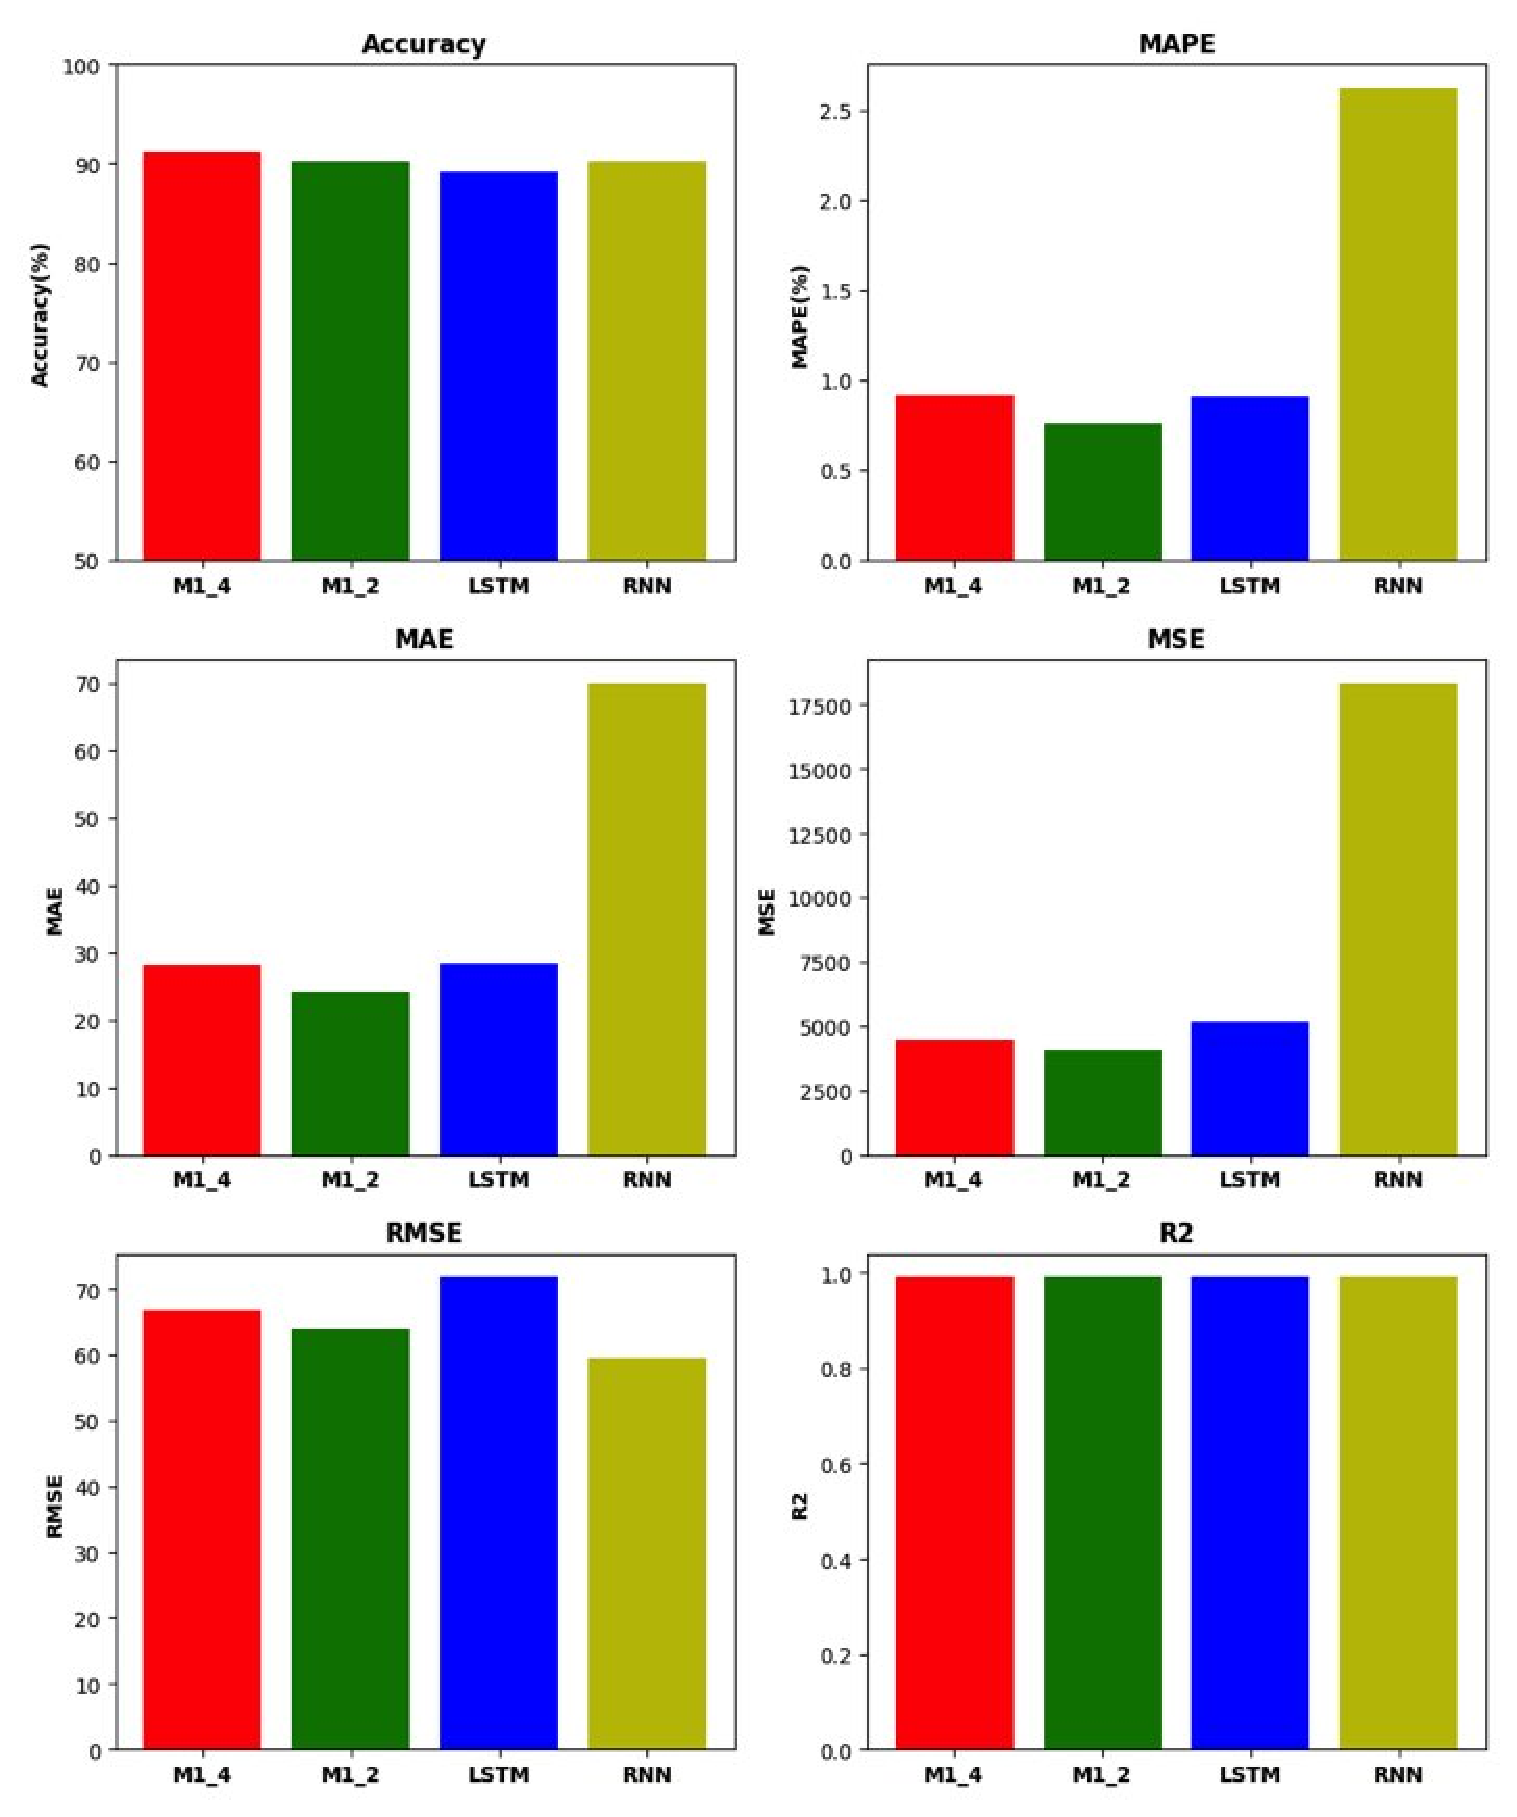
\includegraphics[width=1\linewidth]{images/nasdaq.eps}
	\caption{Comparing metrics among Multi-feature model, Single-feature model,
		LSTM model, and RNN model using NASDAQ as a target.}
	\label{fig:compare1}
\end{figure}

\begin{figure}[H]
	\centering
	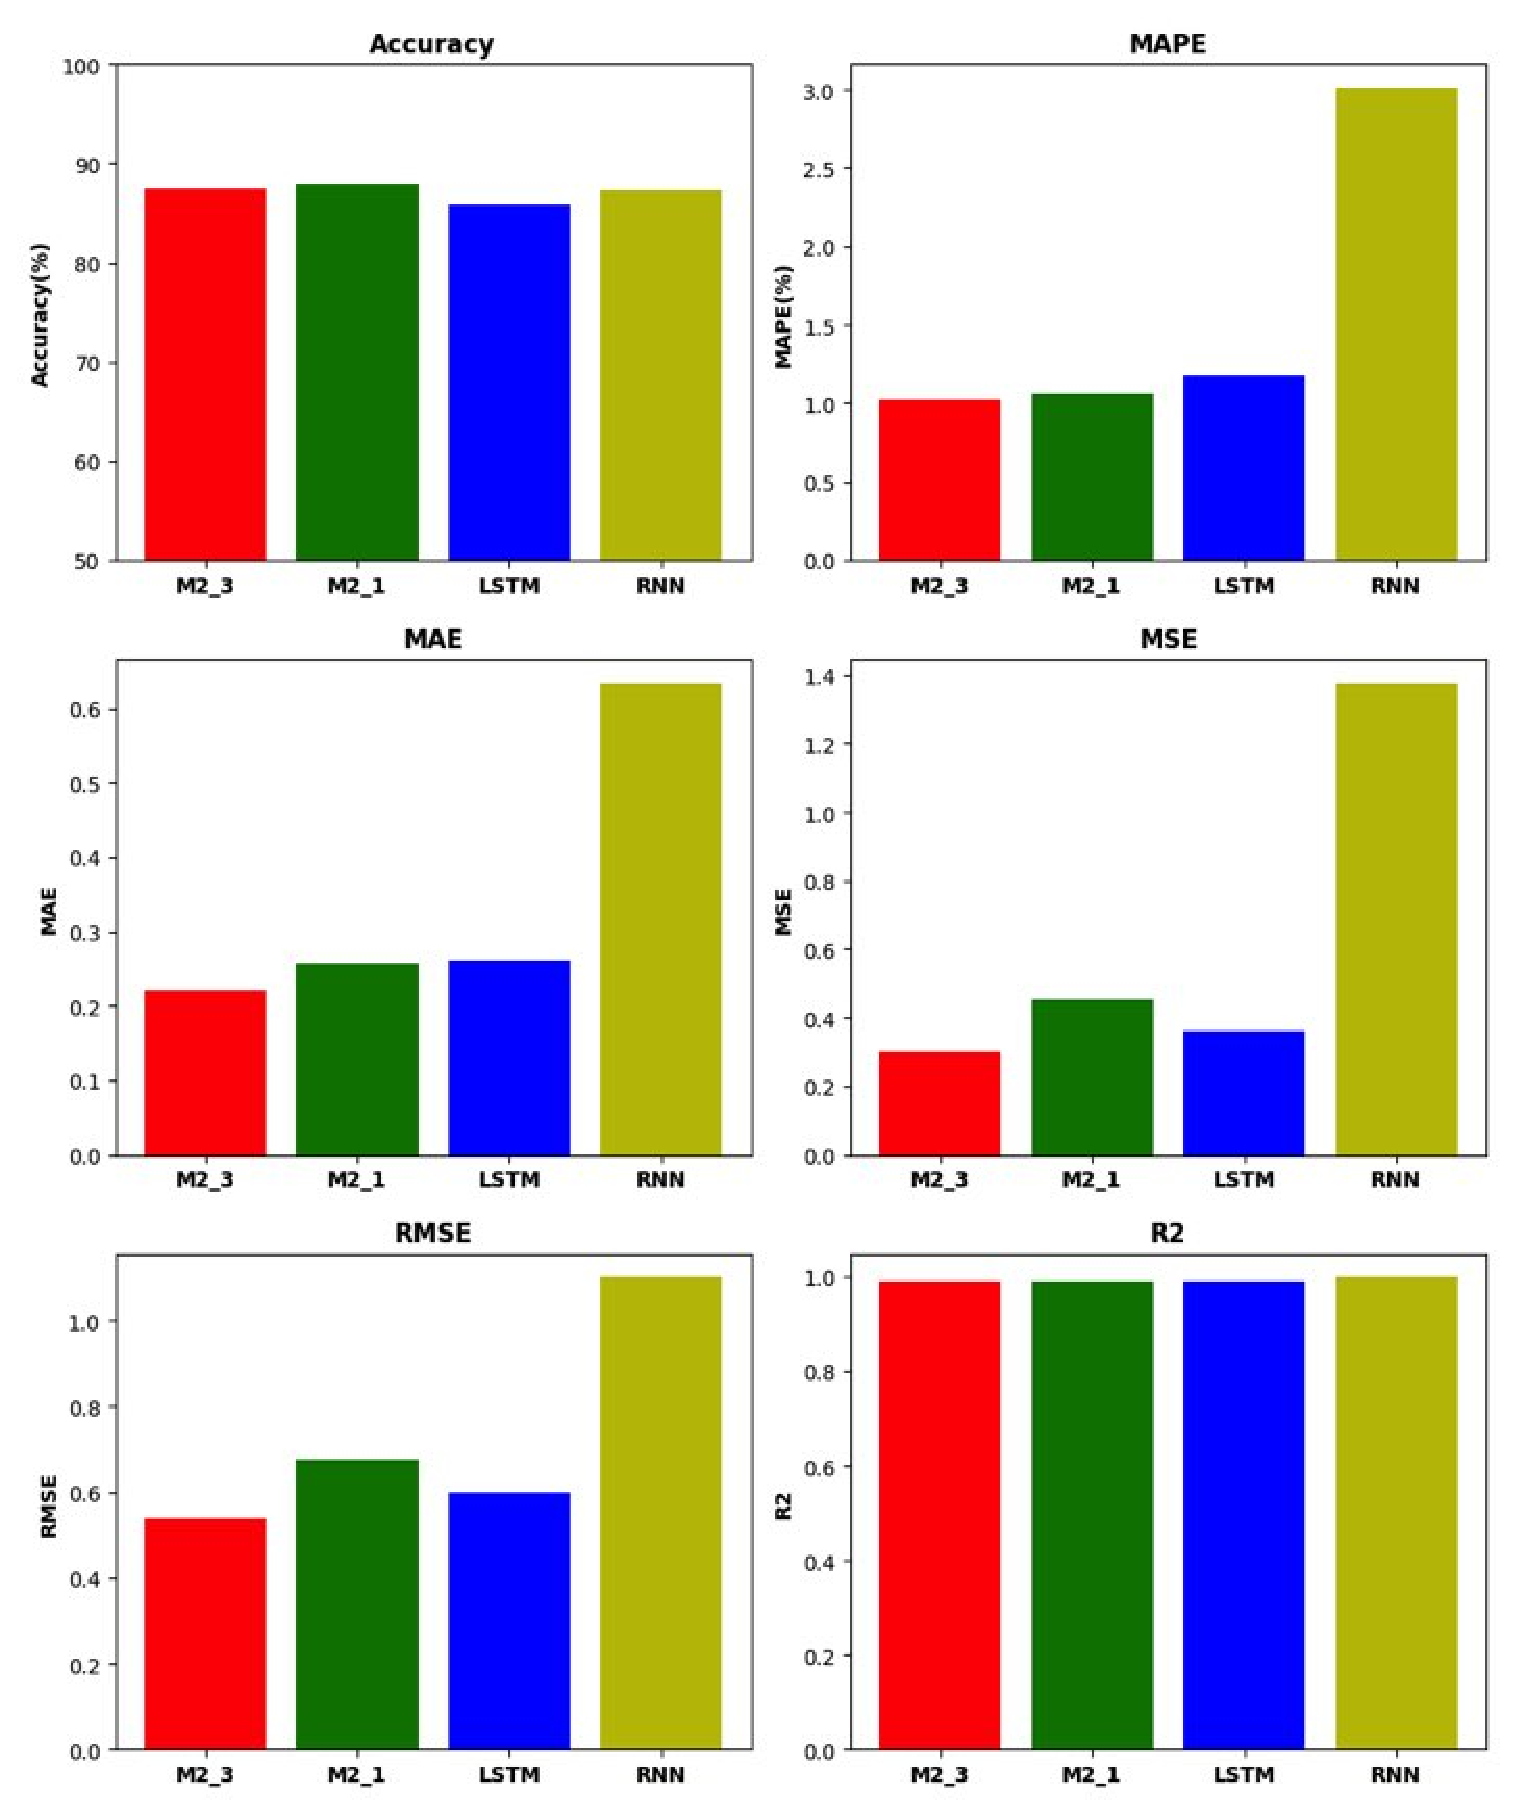
\includegraphics[width=1\linewidth]{images/exxon.eps}
	\caption{Comparing metrics among Multi-feature model, Single-feature model,
		LSTM model, and RNN model using Exxon Mobil as a target.}
	\label{fig:compare2}
\end{figure}